

% The actual figure file is inside common-files/Figs/. Therefore, 
% when this file is inclucded in another tex file located in folder A, 
% a symbolic link should be created inside A/Figs to link the filename
% to the actual figure file inside the common-files/Figs/ folder.
\begin{figure}[htb]
  \begin{center}
        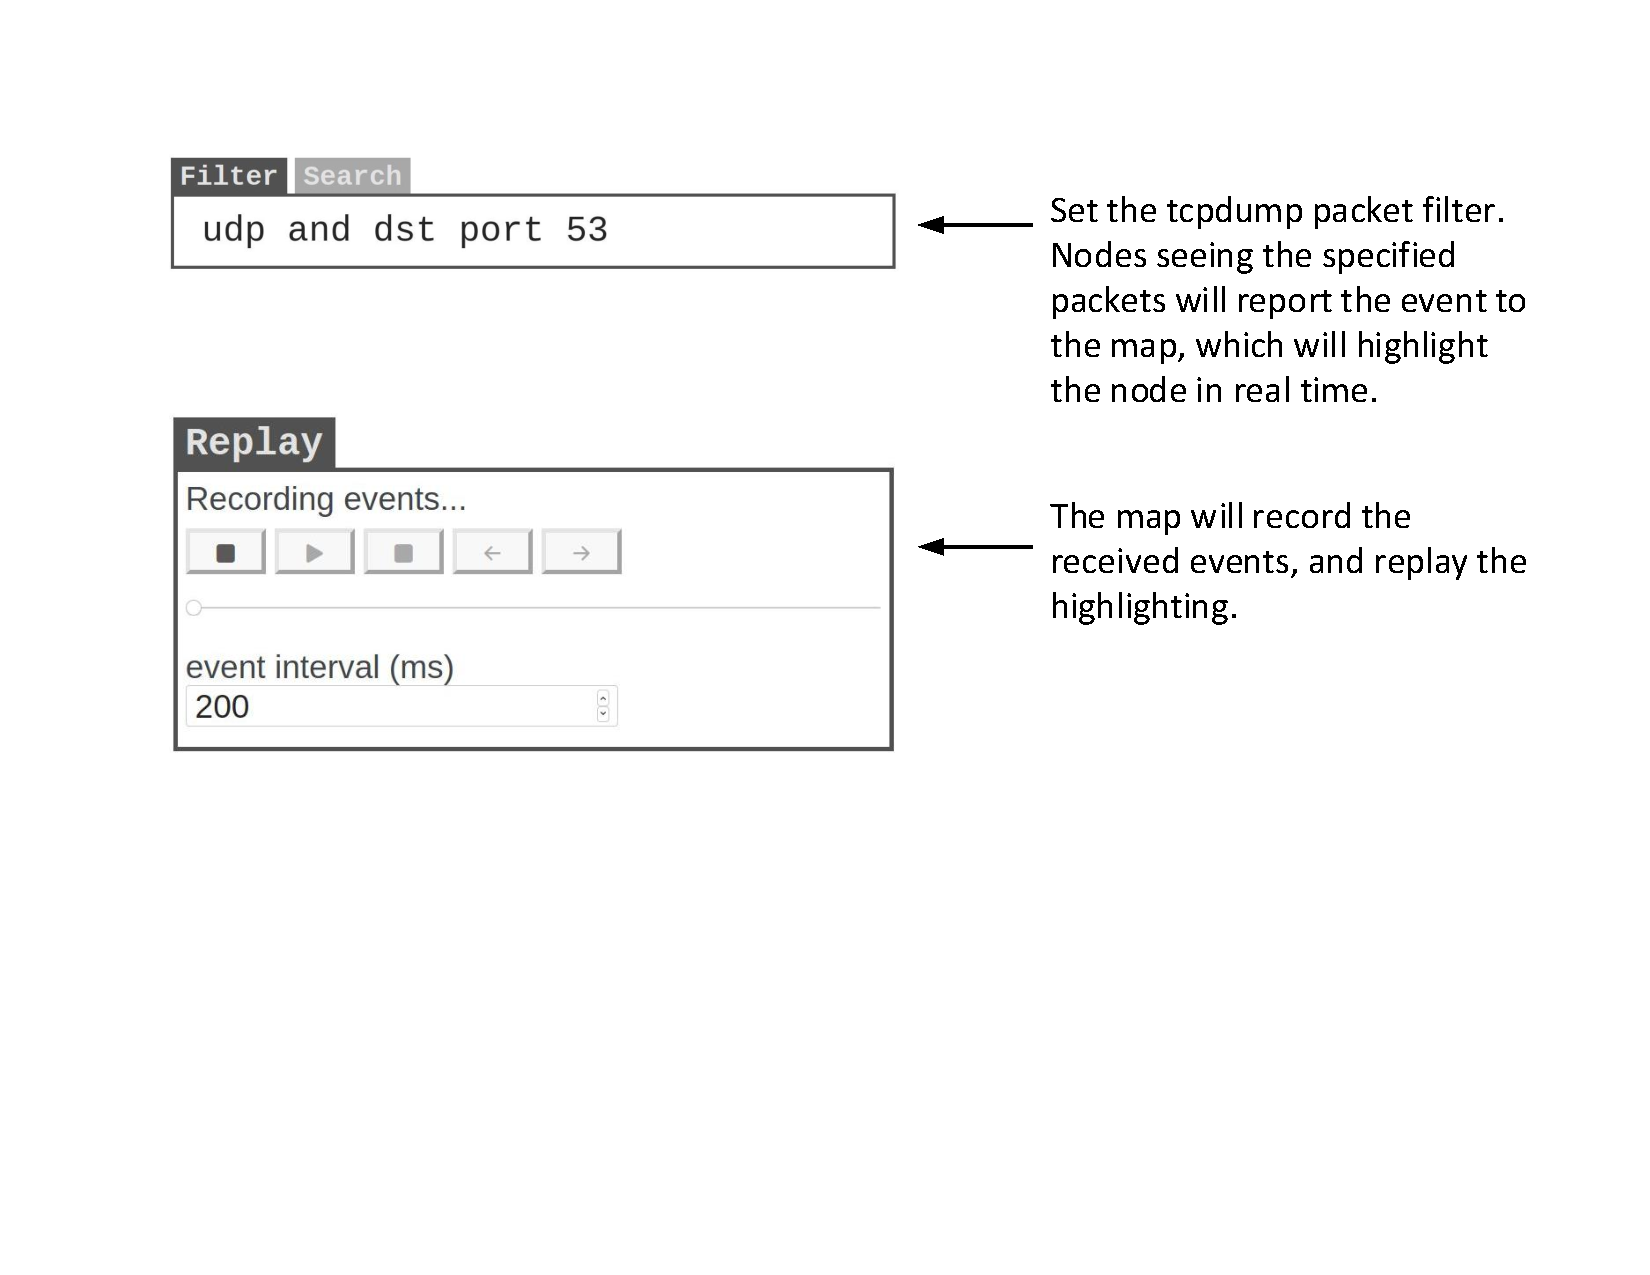
\includegraphics[width=0.6\textwidth]{./Figs/emulator_filter_replay.pdf}
  \end{center}
  \caption{Capturing and replaying events}
  \label{emulator:fig:replay-event}
\end{figure}

Users can also set filters to visualize network traffic.
The syntax of the filter is the same as that in \texttt{tcpdump}; actually,
the filter is directly fed into the \texttt{tcpdump} program running on all nodes.
When a node sees the packets that satisfy the filter, it 
sends an event to the map, which will highlight the node briefly on
the map. 

Sometimes, a sequence of events happen too fast to see the actual order 
among them. In this case, we can use the Replay panel (see 
Figure~\ref{emulator:fig:replay-event}) to record the events and then
replay them at a slower pace. The speed of replaying can be 
adjusted by changing the event interval.


